%!TEX root=../document.tex

\section{Ergebnisse}
\subsection{Theorie}
\subsubsection{iSCSI}
\textbf{Überblick:}\\
\textit{Internet Small Computer Systems Interface} ist eine Erweiterung des \textit{SCSI} Standards. Es erlaubt Clients Daten über TCP in ein \textit{Storage Area Network} (NAS) zu speichern, als wäre es direkt mit der Festplatte verbunden. Damit ist es möglich, mehrere Festplatten von unterschiedlichen Standorten zu einer virtuellen Festplatte zusammenzufassen, welche für mehreren Clients erreichbar ist. Es lassen sich große Distanzen überwinden, da sich iSCSI zwischen Router, host-to-switch, storage-array-to-storage-array implementieren lässt. 

\textbf{Funktionsweise:}\\
iSCSI überträgt block-level Data zwischen iSCSI initiator und den Festplatten, auch iSCSI targets genannt. Der iSCSI initiator kapselt die SCSI Kommandos und Daten in Pakete für den TCP/IP Layer. Diese Pakete werden dann über das Netzwerk mittels point-to-point Verbindung übertragen. Das iSCSI Protokoll trennt dann die SCSI Kommandos von den Daten, so dass es für den Client aussieht, als wäre er direkt lokal mit der Festplatte verbunden.


\textbf{Vorteile:}\\
Der größte Vorteil von iSCSI gegenüber anderen Möglichkeiten, wie FCIP(Fiber Channel over IP), ist, dass keine teuren und komplexen Switches bzw. Router wie für FCIP benötigt werden. Das macht es billiger und einfacher zu verwalten. Weiteres ist iSCSI Variante auch weit flexibler als andere Möglichkeiten. 
\\

\subsubsection{OCFS2}
\textit{Oracle Cluster File System} ist ein verteiltes Dateisystem entwickelt von Oracle Corporation veröffentlicht unter der GNU General Public License. Das Dateisystem ist also eine open source Variante, welche leistungsstarke Performance und hohe Verfügbarkeit bietet. Es verwendet die gleiche Semantik wie lokale Dateisysteme und lässt sich mit jeder beliebigen Anwendung verwenden. 

\subsection{iSCSI Initiator}
Da openfiler bereits zur Verfügung gestellt wurde, musste keine NAS Appliance installiert und konfiguriert werden.

Die restliche Vorgehensweise entspricht genau der Aufgabenstellung. Zuerst wurde das Ubuntu Package \texttt{open-iscsi} installiert. Nachdem in der Datei \texttt{/etc/iscsi/iscsi.conf} die Authentifizierungsmethode auf CHAP (Challenge Handshake Authentication Protocol) gesetzt und die Anmeldedaten konfiguriert wurden, konnte auch schon die Liste der verfügbaren Targets ausgegeben werden.

\begin{lstlisting}[style=bash, caption=Verfügbare Targets]
daniel@daniubuntu:~$ sudo iscsiadm -m discovery -t sendtargets -p 10.0.106.81
10.0.106.81:3260,1 iqn.2006-01.com.openfiler:tsn.96b8938ac933
10.0.106.81:3260,1 iqn.2016-09.syt:tsn.data1
10.0.106.81:3260,1 iqn.2016-09.syt.tgm.data0
10.0.106.81:3260,1 iqn.2006-01.com.openfiler:tsn.465272b2cbcc
10.0.106.81:3260,1 iqn.2016-09.syt:tsn.data0
\end{lstlisting}
Die Option \texttt{-m} legt den Operation-Mode als \texttt{discovery} fest. Im \texttt{discovery} Modus wird mit \texttt{-t} der Discovery-Typ auf \texttt{sendtargets} gesetzt. Mit \texttt{-p} wird die Zieladresse festgelegt.

Danach wurde das \texttt{data0} Target als ``lokale'' Festplatte registriert:
\begin{lstlisting}[style=bash, caption=Target ``lokal'' registrieren]
daniel@daniubuntu:~$ sudo iscsiadm -m node -T iqn.2016-09.syt:tsn.data0 -p 10.0.106.81 --login
Logging in to [iface: default, target: iqn.2016-09.syt:tsn.data0, portal: 10.0.106.81,3260] (multiple)
Login to [iface: default, target: iqn.2016-09.syt:tsn.data0, portal: 10.0.106.81,3260] successful.
\end{lstlisting}
Hier wurde der Modus auf \texttt{node} geändert und mit \texttt{-T} wird der Targetname angegeben. Mit \texttt{-{}-login} wird spezifiziert, dass man sich im \texttt{node} Modus beim angegebenen Target einloggen möchte.

In der Kernel Console sieht man nun das neue Block Device:
\begin{lstlisting}[style=bash, caption=neues Block Device]
[ 1008.354886] sd 33:0:0:0: Attached scsi generic sg2 type 0
[ 1008.369151] sd 33:0:0:0: [sdb] 1048576 512-byte logical blocks: (537 MB/512 MiB)
[ 1008.418559] sd 33:0:0:0: [sdb] Write Protect is off
[ 1008.418605] sd 33:0:0:0: [sdb] Mode Sense: 77 00 00 08
[ 1008.430186] sd 33:0:0:0: [sdb] Write cache: disabled, read cache: disabled, doesn't support DPO or FUA
\end{lstlisting}

\subsection{Client Konfiguration}
\subsection{Server Konfiguration}
\subsection{Testing}
Zuerst wurde mit Client 1 eine Testdatei erstellt. Danach hat Client 2 die Datei geöffnet und bearbeitet.
\begin{figure}[!h]
	\begin{center}
		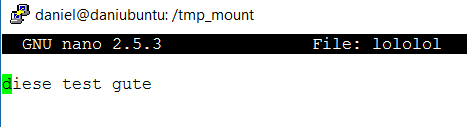
\includegraphics[width=0.5\linewidth]{images/edit.png}
		\caption{Editieren der gemeinsamen Datei}
		\label{edit}
	\end{center}
\end{figure}\

Versucht nun Client 1 ebenfalls die Datei zu editieren erhält man folgende Fehlermeldung:
\begin{figure}[!h]
	\begin{center}
		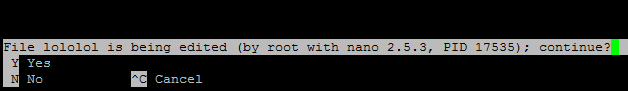
\includegraphics[width=0.8\linewidth]{images/error.png}
		\caption{Gleichzeitiges Editieren}
		\label{error}
	\end{center}
\end{figure}\

Im Endeffekt ist immer die letzte Aktion gültig und überschreibt die vorherigen Änderungen.